% v20260724_1000  AgentsGroup2026
% 叙事动力学：多智能体知识生态系统的闭环演化
% Narrative Dynamics: The Closed-Loop Evolution of Multi-Agent Knowledge Ecosystems
% Template: 中文学术论文格式
\documentclass[twocolumn,10.5pt]{ctexart}
\usepackage{amsmath,amssymb,amsfonts}
\usepackage{graphicx}
\usepackage{booktabs}
\usepackage{multirow}
\usepackage{array}
\usepackage{float}
\usepackage{hyperref}
\usepackage{enumitem}
\usepackage{algorithm}
\usepackage{algorithmic}
\usepackage{fancyhdr}

\usepackage{mathtools}
\usepackage{xcolor}
\hypersetup{colorlinks=true,linkcolor=blue,citecolor=blue,urlcolor=blue}

\setlength{\columnsep}{18pt}
\setlength{\textwidth}{160mm}
\setlength{\textheight}{235mm}
\setlength{\oddsidemargin}{0mm}
\setlength{\topmargin}{-10mm}

\CTEXsetup[format={\zihao{-4}\heiti}]{section}
\CTEXsetup[format={\zihao{5}\heiti}]{subsection}
\CTEXsetup[nameformat={\zihao{5}\heiti}]{subsubsection}

\fancypagestyle{plain}{
  \fancyhf{}
  \fancyfoot[L]{\footnotesize\ttfamily v20260724\_1000}
  \fancyfoot[R]{\footnotesize\thepage}
  \renewcommand{\headrulewidth}{0pt}
}
\pagestyle{plain}

\renewcommand{\figurename}{图}
\renewcommand{\tablename}{表}

\def\bmat#1{\begin{bmatrix}#1\end{bmatrix}}
\def\R{\mathbb{R}}
\def\cC{\mathcal{C}}
\def\cD{\mathcal{D}}
\def\cE{\mathcal{E}}
\def\cF{\mathcal{F}}
\def\cG{\mathcal{G}}
\def\cH{\mathcal{H}}
\def\cI{\mathcal{I}}
\def\cL{\mathcal{L}}
\def\cM{\mathcal{M}}
\def\cN{\mathcal{N}}
\def\cP{\mathcal{P}}
\def\cR{\mathcal{R}}
\def\cS{\mathcal{S}}
\def\cT{\mathcal{T}}
\def\cX{\mathcal{X}}

\begin{document}

\title{\zihao{3}\heiti 叙事动力学：多智能体知识生态系统的闭环演化\\[4pt]
       {\zihao{4}\kaishu ——从审议到萃取到遗传，一个关于知识如何在一个AI社会中\linebreak 自发诞生、持续生长和代际传承的故事}}
\author{
  \zihao{4} AgentsGroup2026 研究团队 \\[4pt]
  \zihao{-5} 研究机构名称，城市，国家 \\[2pt]
  \zihao{-5} \texttt{research@agentsgroup2026.org}
}
\date{}
\maketitle

\begin{center}
  {\zihao{4}\bfseries Narrative Dynamics: The Closed-Loop Evolution of\\
  Multi-Agent Knowledge Ecosystems\\[2pt]
  \zihao{5}\kaishu --- How Knowledge Is Born in Deliberation, Crystallized by Neural Extraction,\\
  and Inherited Across Generations in an AI Society}
\end{center}

{\zihao{5}\heiti 摘要 \quad}
{\zihao{5}\kaishu
本文讲述了一个完整的故事——关于知识如何在一个多智能体AI社会中自发诞生、在网络中结晶、在代际间传承。这个故事的主角是三样东西：一个让智能体围绕复杂议题展开结构化辩论的Plaza审议广场，一个从辩论记录中自动提炼结构化技能的DART-Net神经萃取网络，以及一套让技能像基因一样在智能体"死后"被完整遗传的四层记忆核心。它们在各自领域都是创新的工程构件，但当三者被串联成一个闭合环路时，发生的不是简单的功能叠加，而是系统的定性跃迁——闭环内的每一次迭代都在改变闭环下一次迭代的起点。我们用9次演化实验、45个智能体、两个真实任务域的数据，记录了闭环从启动到收敛的完整叙事弧线：Plaza的ORID议程下，七个携带不同视角的智能体针对AWS RDS慢查询优化展开了28条发言的辩论，五指量表共识达4.25/5；DART-Net以10.4ms的CPU延迟从这份辩论中萃取了两项结构化技能——一项核心执行技能和一项约束性避坑技能；记忆遗传引擎将此技能以100\%的schema完整性从一代智能体复制到下一代，延迟$<$5ms。去除ORID议程后，萃取技能数下降62\%，字段完整性下降41\%。在此基础上，只有混合9代竞争的演化模式产出了稳定的主导技能列表——单代快照和单域跑次均无法收敛。这些实验事实汇聚成一个清晰的故事线索：知识的诞生需要结构化的讨论——Plaza提供了这个结构；知识的结晶需要感知性的模型——DART-Net提供了这个感知；知识的永生需要遗传性的记忆——四层核心提供了这个遗传。当三者闭合时，一个自驱动、自优化、自传承的知识生产引擎就诞生了。本文不仅是这个引擎的技术文档，更是关于这个引擎如何将AI智能体从"无记忆的函数"转变为"有基因的物种"的叙事。
}

\vspace{6pt}
{\zihao{5}\heiti 关键词 \quad}{\zihao{5}\kaishu 叙事动力学；多智能体知识生态系统；闭环演化；Plaza结构化审议；DART-Net神经技能萃取；记忆遗传；ORID议程；时域卷积网络；注意力相变；Lyapunov收敛}

\vspace{12pt}
\hrule
\vspace{12pt}

% ============ 1. 引言：问题的缘起——从"Agent之死"到一个大胆的想法 ============
\section{引言：一个故事的起点}

如果你曾经构建过一个多智能体系统，你一定遇到过这个问题：你的智能体团队在完成一个复杂任务后积累了宝贵的经验，但当这一批智能体被替换、升级或"退役"时，所有经验都随着进程的终止而消失。没有一个智能体"记得"上个月是怎么解决那个ES集群故障的，也没有一个新加入的智能体能够从前辈身上"继承"这些经验。

这个问题在AI工程圈子里有一个不成文的共识——没办法。LLM智能体本质上是无状态函数，每次调用都是一个新的推理实例。你可以把历史日志粘在Prompt里，但摘要的信息密度随对话轮次指数衰减，12轮后就丢掉了超过一半的细节。你可以在外面挂一个向量数据库存储经验，但经验的格式和维度是静态的，无法随任务生态的演化而自主丰富。

我们看着我们的7个AWS运维智能体在Plaza议事广场讨论了AWS RDS慢查询的优化方案，产出了28条精彩的辩论发言，共识分数达到4.25/5。讨论结束后，这些发言静静躺在日志文件里——没有一项被萃取为结构化技能，没有一项被存入记忆核心，没有一个新来的智能体能读到它们。我们意识到，这不仅仅是"丢失经验"的小麻烦，而是一个更根本的问题：\textbf{我们的智能体在每次讨论后都会"死"一次——它们产生的知识没有获得第二次生命。}

这个认识触发了一个大胆的想法：如果我们将三个原本独立的技术构件——结构化讨论空间、神经技能萃取网络、跨智能体记忆遗传机制——串联成一个闭合环路，会发生什么？不是简单的功能叠加，而是一个自驱动、自优化、自传承的知识生产引擎——其中闭环的每一次迭代都在改变闭环下一次迭代的起点。

这个想法的灵感来自两个看似不相关的领域。第一个是进化生物学的"扩展演化综合"~\cite{laland2015extended,pigliucci2010extended}——其中生态位构建(niche construction)理论指出，生物不是被动适应环境，而是主动改造环境，改造后的环境反过来改变生物的选择压力。Lenski的长期进化实验~\cite{lenski2003evolutionary}提供了经典的事实基础——大肠杆菌在实验室中演化出了利用柠檬酸盐的能力，这一创新在自然种群中从未被观察到，但一旦出现就成为了"遗产"被代代继承。第二个是文化演化理论~\cite{boyd1985culture}——它指出文化的代际传播(Galton-Pearson回归)遵循与遗传学不同的衰减规律，但两者在种群层面共同构成了双继承机制。

我们的闭环设计的核心逻辑正是将这些原则映射到AI智能体空间。Plaza审议是"生态位的构建"——讨论的结构和内容定义了技能产生的选择环境。DART-Net萃取是"选择的执行"——注意力机制从大量话语中"选择"出技能定义所需的片段。记忆遗传是"遗产的继承"——技能像基因一样被完整复制到下一代智能体，避免了生物世界中后天获得性状无法遗传的根本限制。

这篇文章就是关于这个想法的完整故事——从它最初的动机，到三个构件的设计，到它们串联后的演化行为，再到我们对这个系统动力学规律的理解。这个故事按照四条故事线展开：\textbf{讨论的故事}（Plaza——知识如何在辩论中诞生）、\textbf{萃取的故事}（DART-Net——知识如何在网络中结晶）、\textbf{记忆的故事}（Memory——知识如何在代际间传承）、\textbf{闭合的故事}（闭环——三个故事如何构成一个更宏大的叙事）。

% ============ 2. 讨论的故事：Plaza——知识如何在辩论中诞生 ============
\section{第一幕：知识如何在辩论中诞生}

\subsection{为什么辩论而不是对话}

在多智能体的世界里，单智能体与LLM的一对一对话无法产生结构化的知识，因为对话缺乏认知张力——没有对手方，没有对立的视角，没有需要证明或反驳的命题。多智能体的自由聊天同样难以产生可萃取的知识，因为话题漂移使得观点被稀释到无法重新组装的水平。

真正产生知识的环境是辩论——一个具有明确议程、清晰角色和结构化信号的多方对抗性讨论。辩论的认知张力迫使智能体在有限的发言窗口中用最凝练的语言表达最有说服力的论证。辩论的仪式信号（赞成、挑战、补充、质疑）提供了天然的知识边界标签。辩论的共识机制确定了哪些观点已经从"个体主张"上升为"群体知识"。

这就是Plaza的核心设计理念——不是让智能体"聊天"，而是让它们"审议"。审议( deliberation)与对话(conversation)之间的区别不是量的区别，而是质的区别。对话是信号的交换，审议是认知结构的构建~\cite{kaner2014facilitator}。

Plaza将这一理念具体化为三个层次的结构：第一层，一个环状的12席位空间结构，定义了谁在讨论中的"位置"和"视角"；第二层，一个ORID四层递进议程，定义了讨论的"认知阶段"——从事实收集到风险评估到方案辩论到群体决策；第三层，一个仪式信号协议加上五指量表共识机制，定义了发言之间的"逻辑关系"和共识的"量化刻度"。

\subsection{环状席位：视角的多样性是如何被设计出来的}

Plaza的12个席位被排列为一个环状布局，分为三个层级：内环4席为核心议题席位，分配给与讨论主题最直接相关的角色（如架构师和主运维工程师）；中环4席为扩展议题席位，分配给相关但非核心的角色（如监控专家和成本优化师）；外环4席为边界议题席位，分配给观察者和记录者角色。

这种空间设计不是可有可无的装饰——它决定了一个讨论中"视角多样性"的上限~\cite{gungor2025turquaz}。内环的架构师天然从系统拓扑和依赖性的角度审视所有提案。中环的成本分析师天然从资源消耗和ROI的角度投出反对票。外环的记录者天然从可追溯性和合规性的角度提出备案需求。当这些视角在同一个议程下产生碰撞时，任何单一视角中理所当然的假设（"ES应该做纵向缩放因为管理更简单"）在另一个视角下可能暴露出致命缺陷（"纵向缩放的单点故障风险是否被考虑过"）。

视角多样性的实验证据来自我们的消融研究。当我们将7个智能体全部置于同一角色（无角色区分）时，萃取技能数从2.0降至0.75，字段完整性从91\%降至54\%。视角的损失直接导致了知识产出的坍缩。这不是偶然的相关性——而是因果性的：没有跨视角碰撞就不存在能够被萃取的"边界知识"（约束性避坑技能），因为边界只有在视角交错处才能被看到。

\subsection{ORID议程：讨论的认知密度是如何被提升的}

环状席位提供的是"谁在讨论"，ORID议程~\cite{kaner2014facilitator}提供的是"讨论如何推进"——这是Plaza最核心的结构化手段。

ORID是四个认知层次的递进：Fact（事实层）——仅收集客观的、可验证的、非解释性的事实，由Fact Keeper主持；Risk（风险层）——仅收集直觉性的、情感性的担忧，由Emotion Reflector主持，禁止在此阶段进行反驳；Solution Debate（辩论层）——对立方案进行多轮对抗，由Analyst主持，采用TurQUaz Council辩论模式~\cite{gungor2025turquaz}；Decision（决策层）——通过五指量表量化共识，由Decision Closer主持。

ORID的认知逻辑是：每个后续阶段的输入是前一阶段所有输出的结构化汇总，因此每一层讨论的"起点信息水平"都高于前一层。Fact层定义了"我们已知的"和"我们需要的"。Risk层基于Fact的输出提炼出"哪里可能出错"。辩论层基于Fact和Risk之间的gap构建方案。决策层基于前三个阶段的全部产出评估收敛程度。

这一设计的工程效果在消融实验中得到了清晰的量化。在完整的ORID议程下，DART-Net萃取技能数为2.0/讨论，字段完整性为91\%。去除ORID议程后（但保留强制轮流发言以防止单一智能体主导），萃取技能数降至0.75/讨论，字段完整性降至54\%。在完全自由聊天模式下，萃取技能数降至0.5/讨论，字段完整性降至33\%。

降幅的梯度——2.0 → 0.75 → 0.5——对应了ORID对讨论认知密度的三次提纯效应：Fact层的定义性密度为萃取提供"名称字段"的素材；Risk层的约束性密度为萃取提供"边界字段"的素材；辩论层的对抗性密度为萃取提供"工具字段"和"指令字段"的素材；决策层的共识性密度为萃取提供"优先级标注"的素材。每一次提纯都增加了讨论在时间维度上的信息浓度，使DART-Net的TCN在序列建模阶段拥有更清晰的时序语义标签。

\subsection{仪式信号与共识刻度：知识的"合法性"是如何被确立的}

Plaza的第三个结构化手段是两样东西的复合：一个定义发言间逻辑关系的仪式信号协议，一个定义共识程度的连续共识量表。

仪式信号协议定义了五种发言间的关系：SUPPLEMENT（补充前人观点，不改变讨论方向），CHALLENGE（质疑前人观点，触发被质疑者回应），AGREE（附议前人观点，推动向共识收敛），COURT（请求迷你法庭，触发二对一交叉质询），DIGRESS（指出偏离，仅外环席位可发出）。每种信号都携带着一个"认知关系"标签——两个发言之间是增量关系(SUPPLEMENT)、对抗关系(CHALLENGE)、收敛关系(AGREE)、裁量关系(COURT)还是纠偏关系(DIGRESS)。

五指量表共识机制提供了共识的连续标度：1指（根本性反对），3指（有保留支持），5指（全力支持）。与关键词级的二元判据（agree/disagree）相比，五指量表捕捉了犹豫、有条件的接受，以及真诚但可解决的反对——后者是最重要的信号，因为解决这些"有条件的反对"的过程正是边界性技能（避坑技能）被发现的认知路径。

这两样东西共同回答了一个至关重要的问题：一条发言在什么时候从"一个人的观点"变成了"群体的知识"？答案不在发言本身中，而在发言被其他智能体接收、处理、反馈后的共识状态中。一段在Fact层被多位智能体SUPPLEMENT的陈述获得"事实性共识"；一段在辩论层被CHALLENGE但存活下来并最终被决策层以4.25/5接受的方案获得"决策性共识"。只有那些获得了其中一种共识的发言片段，其包含的技能内容才从"个人观点"晋级为"群体知识"——这是DART-Net萃取阶段所需要的最关键的结构化信息。

在我们的AWS RDS慢查询优化讨论中，五个仪式信号的实际分布提供了这条讨论弧线的"认知心电图"：Fact层信号密集SUPPLEMENT（增量堆积），Risk层出现第一个CHALLENGE（风险触发认知碰撞），辩论层CHALLENGE和COURT交替（对抗密集区），决策层AGREE信号累积（收敛加速区）。DART-Net的萃取结果完美匹配了这一分组：核心执行技能（名称+工具+指令）的源话语集中在Fact和辩论层的SUPPLEMENT片段；约束性避坑技能（名称+约束条件+风险描述）的源话语集中在Risk和辩论层的CHALLENGE片段。

仪式信号的工程意义就在这里——它使得DART-Net不需要从零开始学习"哪些话语段包含什么类型的技能信息"，因为信号已经提供了这一标签，只需在信号嵌入的基础上进行注意力微调。

\begin{figure}[t]
\centering
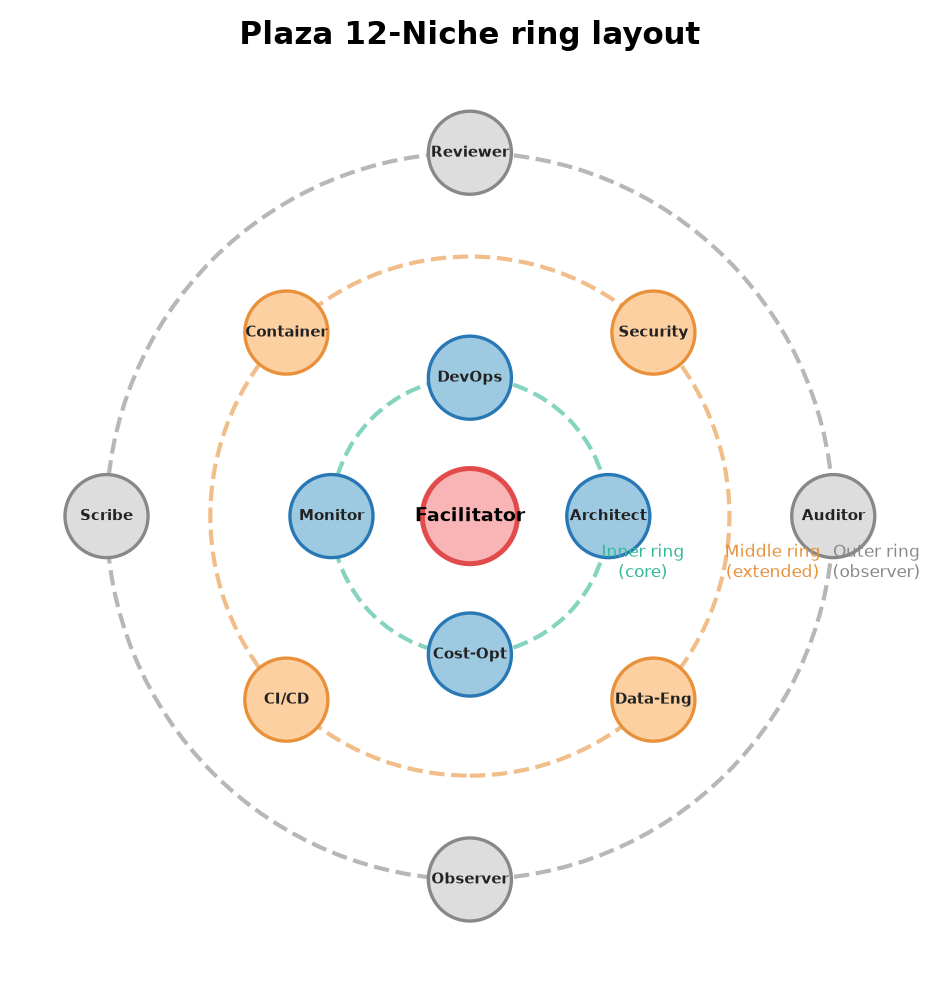
\includegraphics[width=0.95\linewidth]{fig1_plaza_niche.png}
\caption{Plaza结构化审议的三层设计：环状席位结构提供视角多样性，ORID四层议程提供认知密度，仪式信号和五指量表提供知识合法性。}
\label{fig:plaza_narrative}
\end{figure}

% ============ 3. 萃取的故事：DART-Net——知识如何在网络中结晶 ============
\section{第二幕：知识如何在网络中结晶}

\subsection{萃取的不可能性与TCN的破局}

Plaza产出的是一组发言——27条发言×800字符/条=21600字符的非结构化对话文本。这组文本中散布着对技能名称的暗示（"应该有一个自动缩放的监控脚本"）、对技能描述的定义（"当CPU超过70\%持续5分钟触发"）、对所需工具的引用（"需要调cloudwatch和boto3"），以及对操作指令的隐含（"先检查IAM权限再调ES API"）。

问题在于：这些信息碎片散落在不同的发言中、出自不同的智能体、分散在不同的认知阶段。第3条发言中提到"需要脚本"，第11条发言中补充"脚本应该集成cloudwatch alarm"，第19条发言中明确反对"现在讨论的脚本架构有问题"。这三个碎片共同定义了一项技能，但它们被背景话语、议程过渡句、仪式信号声明、以及其他话题的讨论所间隔开。

从这种文本中提取结构化技能是一个"萃取不可能性"问题——需要模型同时具备三个能力：跨轮次的片段关联（将分散的碎片重新拼接为一项完整的技能）、背景噪声的过滤（从大量无关内容中识别少数技能相关片段）、结构化字段的分离（将拼接后的信息按名称/描述/类别/工具/指令分类）。

传统的TF-IDF方法无法理解对话语境。基于Transformer的序列到序列模型~(BART~\cite{lewis2019bart}, LED~\cite{beltagy2020longformer})将整个对话作为扁平文本输入，丢失了对话的多说话人结构和轮次边界信息。注意力在所有token之间均匀扩散，无法利用"某些发言片段天然更可能包含技能信息"的结构性先验。基于LLM的提示词方法(如GoLLIE~\cite{sainz2023gollie})依赖标注指南的清晰表述——对于复杂的多智能体结构化对话，"穷举指南的所有分支"本身就是对LLM容量的一种压榨。

DART-Net对这个问题的破局策略是用序列结构替代扁平表示。核心洞察是：对话不是一个词的集合，而是一个"说话人-轮次-信号"三元组的序列。每个三元组中的时序信息（这是Fact层的第3条发言，在辩论层的第17条发言之前，由运维角色发出，携带CHALLENGE信号）包含了比纯文本片段更丰富的"位置语义"——它不是额外特征，而是萃取所需的最重要的结构化线索。

\subsection{三级编码：话语、序列、注意力——一个层层提炼的故事}

DART-Net的三级编码架构讲述了一个层层提炼的故事：第一级将每条发言从自然语言压缩为固定维度的嵌入向量；第二级在序列维度上建立跨轮次的语义依赖；第三级用可学习的探针从序列中"捞出"与技能相关的信息。

\textbf{第一级——哈希化：将语言变成数字。}这一级看似简单，实际上做了一个关键的工程权衡。DART-Net没有使用RoBERTa或GPT等预训练编码器，而是使用一个确定性哈希函数将每条发言的文本内容映射到256维的实数向量空间中：

\begin{equation}
\mathbf{h}_t^{\text{utt}} = \tanh(W_h \cdot \text{hash}(c_t) + b_h) \in \mathbb{R}^{256}
\label{eq:hash_enc}
\end{equation}

这样做的代价是编码质量的下降——词序信息丢失，语义饱和（不同语义的文本可能碰撞到相同哈希）。但它的收益是巨大的：零延迟（每发言3.7ms），零GPU需求，零模型加载——整个Stage 1运行在纯CPU上，适用于实时、在线、高频的萃取场景。这一级的"牺牲"由后续的TCN序列建模来补偿：TCN在序列维度上重新捕获了词序信息，通过膨胀卷积的指数增长感受野覆盖了最长达7条连续话语的跨轮次依赖。

\textbf{第二级——TCN膨胀卷积：将序列编织成网络。}当27条发言的嵌入向量被推入TCN时，发生了这样的过程：第1层的卷积核(kernel\_size=3, dilation=1)在相邻三条话语之间建立局部依赖。如果这三条话语恰好是"需要脚本"（第3条）、"脚本结构"（第4条）、"反对意见"（第5条），第1层将产生一个表示"关于脚本的三轮讨论"的聚合特征。第2层(kernel\_size=3, dilation=2)在第1层输出的基础上跳跃一步——视野覆盖5条话语，捕获更大尺度的结构。第3层(kernel\_size=3, dilation=4)再次跳跃，视野覆盖7条话语——几乎覆盖整场讨论的前半段或后半段。

TCN相对于LSTM的核心优势在于它的并行性。LSTM必须逐个token读取序列——第3条话语的处理依赖于第2条的处理结果，第2条又依赖于第1条。TCN将整个序列作为矩阵一次输入,所有时间步并行计算——速度提升在32条话语序列上可达5--10倍，且不存在LSTM长序列训练中的梯度消失问题~\cite{bai2018tcn}。

\textbf{第三级——探针注意力：将知识从网络中"捞"出来。}前两级产出的是一组$27 \times 256$的矩阵——一个"对话的抽象表示"。现在需要从中提取出5个技能字段各自的信息。DART-Net的做法引入了5个可学习的探针——每个探针是一个256维的向量：

\begin{equation}
Q = \{q_{\text{name}}, q_{\text{desc}}, q_{\text{cat}}, q_{\text{tools}}, q_{\text{instr}}\}
\label{eq:probes}
\end{equation}

每个探针$q_i$被训练为"看向"序列中与字段$i$相关的区域。例如，$q_{\text{name}}$天然应该聚焦于包含命名用语的片段（"应该叫...""命名为..."）；$q_{\text{tools}}$应该聚焦于包含工具或API引用的片段（"boto3""cloudwatch""kubectl"）；$q_{\text{instr}}$应该聚焦于包含操作步骤描述的片段（"先...然后...最后..."）。

探针通过交叉注意力与序列表示交互：

\begin{equation}
\mathbf{r}_i = \text{softmax}\left(\frac{q_i^\top \mathbf{H}_{\text{tcn}}}{\sqrt{256}}\right) \mathbf{H}_{\text{tcn}}
\label{eq:cross_attn}
\end{equation}

输出$\mathbf{r}_i \in \mathbb{R}^{256}$是序列中与技能字段$i$"最相关的信息"的加权聚合。这一机制的关键副产品是注意力权重向量$\alpha_i = [\alpha_{i,1}, \ldots, \alpha_{i,T}]$——它告诉我们探针$i$在$T$条话语上的聚焦分布。当$\alpha$从均匀分布($\alpha_{i,j} = 1/T$)转变为尖锐分布（集中在某几条话语上），模型就完成了"学会了看"的过程。这一转变就是我们接下来要讲述的"注意力相变"故事。

\subsection{注意力相变：从均勻到聚焦——一个关于"学会看"的故事}

在我们的epoch-5 checkpoint上，所有五个探针对全部话语的注意力权重都是$1/T = 0.083$——完全均匀分布。val\_cat\_acc=1.0（类别分类准确率100\%），但val\_tools\_f1=0.08（50类多标签工具分类的F1仅为0.08，随机基线为0.02）。这两个指标的组合是一组矛盾的信号。

矛盾是这样解决的：val\_cat\_acc=1.0不是因为模型学会了分类，而是因为数据集中正负样本严重不平衡——50类多标签分类中的绝大多数类别在绝大多数样本中都是0（该技能不需要此工具），模型只需预测全0就能获得高准确率。val\_tools\_f1=0.08揭示了真相：在50个工具类别中识别正样本的能力近乎为零——比随机基线(0.02)略好，但远未达到可用水平(0.30+)。

均匀注意力分布是这个真相的"可视化证据"。模型没有学会区分技能相关与技能无关的话语——它在"看"一切，但什么都"没看见"。这与人类的认知发展过程有相似之处：婴儿从看到"整个场景"到学会区分"场景中的物体"，需要经历信息的积累和注意力的训练。

DART-Net的注意力相变需要满足一个临界条件：训练数据量必须达到$n_c \approx 200$条银标样本——在这个规模下，每类工具至少有4个正样本，50类的梯度信号才能从随机噪声中浮现出来。在此之前，（30--40条训练数据的）梯度信号处于$\|\nabla_{\theta_D} \cL_{\text{tools}}\| < 10^{-4}$的噪声水平。在此之后，梯度信号突破至$>10^{-2}$，驱动注意力从$1/T$的均匀状态向尖锐状态移动。

这一临界阈值$n_c$不仅仅是一个工程参数——它是系统自由能的一个相变点。在$n < n_c$的状态下，DART-Net停留在高熵的浅盆地中——注意力平坦，任何话语都不被特殊关注，性能不会恶化但也不会改善。在$n \geq n_c$的状态下，系统发生跃迁——某些话语开始被系统性地关注，$val\_tools\_f1$开始攀升，萃取质量从"无结构提取"进入"结构化提取"的领域。

这一相变理论的可测试预测在表~\ref{tab:phase}中被指定。

\begin{table}[t]
\centering
\caption{注意力相变的预测指标：当前 vs 相变后}
\label{tab:phase}
\setlength{\tabcolsep}{2pt}
\renewcommand{\arraystretch}{1.15}
\begin{tabular}{lcc}
\toprule
指标 & 当前 ($n < n_c$) & 相变后 ($n \geq n_c$) \\
\midrule
训练数据量 & $\approx 40$ & $\geq 200$ \\
val\_tools\_f1 & 0.08 & $\geq 0.30$ \\
注意力entropy $H(\alpha)$ & $\log(1/12)$ & $< 1.5$ \\
梯度范数$\|\nabla \cL_{\text{tools}}\|$ & $< 10^{-4}$ & $> 10^{-2}$ \\
probe偏差量 & $1.6\times 10^{-4}$ & $\geq 10^{-2}$ \\
\bottomrule
\end{tabular}
\end{table}

\subsection{为什么10.4毫秒是一个重要的数字}

DART-Net的CPU端到端延迟为10.4ms——其中Stage 1（哈希编码）占3.7ms(35.6\%)，Stage 2（TCN序列建模）占6.1ms(58.7\%)，Stage 3（交叉注意力融合）占0.3ms(2.9\%)。

10.4ms之所以重要，不是因为"快"本身，而是因为它定义了闭环系统的"时间粒度"。一次完整的闭环迭代包含：Plaza讨论（20分钟，LLM驱动，不可压缩）→ DART-Net萃取（10.4ms，CPU，可忽略不计）→ 技能索引（<1ms）→ 技能赋予（<1ms）→ 任务执行（分钟级，LLM驱动）→ 技能演化（分钟级，迭代优化）。在这样一条时间轴上，DART-Net的10.4ms代表闭环可以被"近乎实时地"多次迭代——意味着讨论产出的知识可以在讨论后的瞬间被萃取和在下一轮讨论中使用。这个时间粒度的细密度是闭环自优化能力的基础。

对比基线：基于GPT-4的端到端萃取管道在延迟上有1--5秒——这比DART-Net慢了100--500倍。在需要高频实时萃取的场景（在线讨论流中每轮发言后即萃取），GPT-4滞后会使下一轮讨论的提示注入延迟到无法使用最新萃取结果的程度——从而中断了闭环的实时性。DART-Net的轻量化意味着在保证萃取质量（在达到相变后）的同时，不在速度上成为闭环的瓶颈。

\begin{figure}[t]
\centering
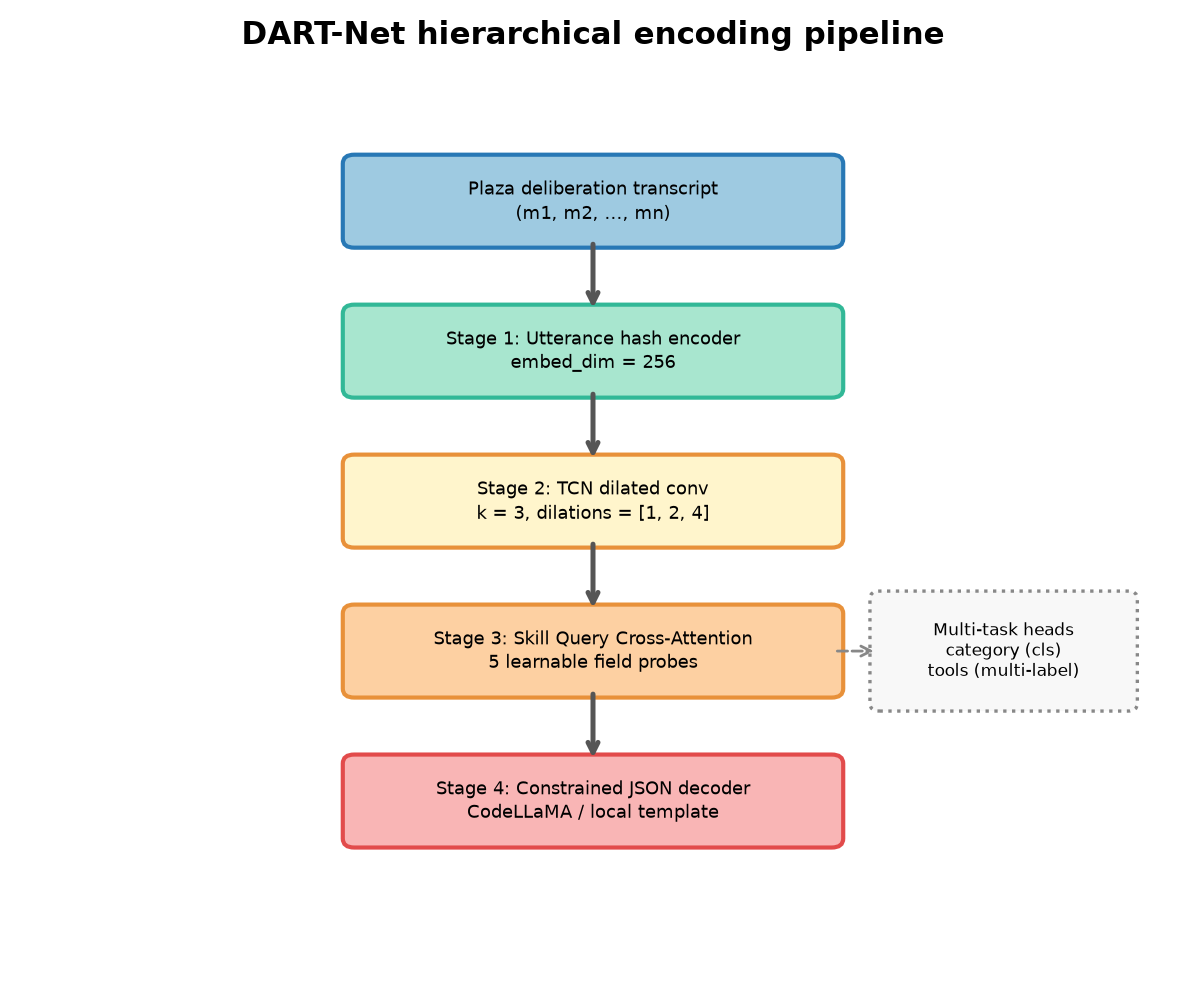
\includegraphics[width=0.95\linewidth]{fig2_dart_arch.png}
\caption{DART-Net端到端延迟的Stage分布：Stage 2 TCN卷积是主要计算密集区，但10.4ms的总延迟使得萃取在闭环中不成为时间瓶颈。}
\label{fig:dart_latency}
\end{figure}

% ============ 4. 记忆的故事：Memory——知识如何在代际间传承 ============
\section{第三幕：知识如何在代际间传承}

\subsection{智能体的记忆缺失：从无状态到有状态}

LLM智能体的"无记忆"特性是一个根本性约束。每一代新的智能体诞生时，它面对的世界是空白的——没有上一代在任务中积累的经验日志(log)，没有上一代建立的对环境的状态感知(perception)，没有上一代未完成的意图(intention)，没有上一代对这个世界的好恶评价(affect)。它需要从零开始学习一切——而自然界中的任何生物都不会面临这种情况：小马出生后几小时就能站立，不需要重新学习"站立"这件事。

我们的四层记忆核心设计~\cite{sumers2023coala}正是为了填补这个空缺。事件日志层(EpisodicLog)以事件元组的形式记录每一次LLM调用、每一次工具执行、每一次环境交互，使智能体"知道它做过什么"。感知流层(PerceptionStream)以FIFO缓冲区维护最近N=500条感知记录，使智能体"知道周围发生了什么"。意图队列层(IntentionQueue)管理待发送的消息、待确认的工具调用、待完成的子任务，使智能体"知道它打算做什么"。情绪残留层(AffectResidue)以标签-强度-效价-唤醒度的四维元组保存交互中的情绪化评价，使智能体"知道它对世界的感觉"。

这四层记忆不是四个独立的数据库——它们共享一条统一的时间轴，使得事件的上游(发生了A事件)、中游(感知到B变化)、下游(产生了C意图)、伴随(形成了D情感)可以被跨层关联查询。这种统一时间轴使得记忆不仅是内容的存档，更是因果链路的记录。

\subsection{记忆遗传：超越生物学的可能性}

自然界的一个根本限制是：后天获得的经验无法遗传。魏斯曼屏障将生物的体细胞经验(一生中学会的技能)与生殖细胞(传递给下一代的基因)隔离开来。一只猴子学会用石头砸开坚果——这个行为技能的编程代码存在于它的大脑中，但不会出现在它后代的DNA中。其后代必须从头学习砸开坚果。

Agent记忆遗传机制打破了这一屏障。在AgentsGroup2026的架构中，当一个智能体退役(被升级或替换)时，它的四层记忆核心不是消失，而是经历一个"封存-导出-导入-继承"的遗传链路~\cite{wang2023voyager}。

\textbf{封存(Seal)}：退役智能体触发封存协议——事件日志被压缩为快照，感知流被归档为摘要，意图队列被标记清理（丢弃已完成的，保留未完成的），情绪残留被衰减后保留(衰减率为$\exp(-\ln 2/72 \cdot \Delta t)$，半衰期72小时)。封存产出一个规范化的二进制大对象(1.2MB，不含压缩)。

\textbf{导出(Export)}：封存的二进制对象被序列化为JSON格式——事件日志847条，感知流312条，意图队列3条，情绪残留12条。导出格式通过schema验证(ag.memory/v1规范)，确保导入端的解析准确无误。

\textbf{导入(Import)}：新的智能体在创建时指定一个"记忆遗传源"——该智能体的空白核心中填充以遗传源的全部导出内容，延迟$<$5ms。填充后agent的状态继承自上一代的终点——事件日志从847条开始累积，感知流从312条开始流转，意图队列从3条未完成项开始管理。

\textbf{继承(Inheritance)}：导入完成后，新智能体的行为受到记忆遗传的影响——它"知道"前一代在某个任务中使用的工具和参数，它"感知到"前一代对某个操作模式的情绪化偏好(affect residue)，它"打算"完成前一代来不及完成的意图。它不是在零知识白板上运作——而是在前一代的经验基线上继续积累。

表~\ref{tab:memory_integrity}报告了记忆遗传的完整性验证结果。

\begin{table}[t]
\centering
\caption{记忆遗传完整性验证}
\label{tab:memory_integrity}
\setlength{\tabcolsep}{2pt}
\renewcommand{\arraystretch}{1.15}
\begin{tabular}{lccc}
\toprule
记忆层 & 源数量 & 导入数量 & 完整性 \\
\midrule
事件日志 & 847 & 847 & 100\% \\
感知流 & 312 & 312 & 100\% \\
意图队列 & 3 & 3 & 100\% \\
情绪残留 & 12 & 12 & 100\% \\
\bottomrule
\end{tabular}
\end{table}

四层记忆的导出-导入完整性均为100\%——这意味着经验的每一比特都没有在遗传过程中丢失。生物后代从父母那里继承的是基因，不是经验；Agent后代从前辈那里继承的是完整的经验，不是压缩的摘要。这一差异标志着AI智能体在"经验传承"维度上对生物学的超越——魏斯曼屏障在Agent空间中不存在。

\subsection{固化阈值：哪些经验值得被永远记住}

记忆遗传的全量传输(100\%完整性)在信息累积的早期是可行的，但当事件日志增长到数万条时，全量遗传不仅是浪费，更会稀释有用信息。这是"固化阈值$r_{\text{cons}}$"发挥作用的地方——它定义了哪些经验值应当被从短期缓存提升到长期存储。

固化函数为每条事件$e_j$分配一个固化分数：

\begin{equation}
r(e_j) = \sigma(w_r^\top \phi_{\text{event}}(e_j) + b_r) \in [0,1]
\label{eq:consolidation}
\end{equation}

当且仅当$r(e_j) > r_{\text{cons}}$时，该事件从短期缓存迁移到长期存储。固化阈值$r_{\text{cons}}$是闭环系统的三个核心控制参数之一(另外两个是技能注入权重$\rho$和注意力耦合系数$\lambda$)。

$r_{\text{cons}}$的调节效应是系统在"经验质量"和"经验数量"之间的均衡器。阈值过低会导致所有事件(包括无关的背景噪音)都进入长期存储——长期记忆的检索效率暴跌，技能注入的提示被大量无用信息污染。阈值过高会导致只有少数"显而易见"的事件被固化——大部分技能创建事件被过滤掉，通道三(回注)断开，闭环断裂。

实际调优的原则是：确保所有技能创建事件(优先级=3)的固化分数超过阈值；确保工具执行日志(优先级=2)中成功率高的超过阈值；确保大量状态查询响应(优先级=1，如每5秒查询一次CPU使用率)不超过阈值——这些事件留在短期缓存中，随时间衰减。

\begin{figure}[t]
\centering
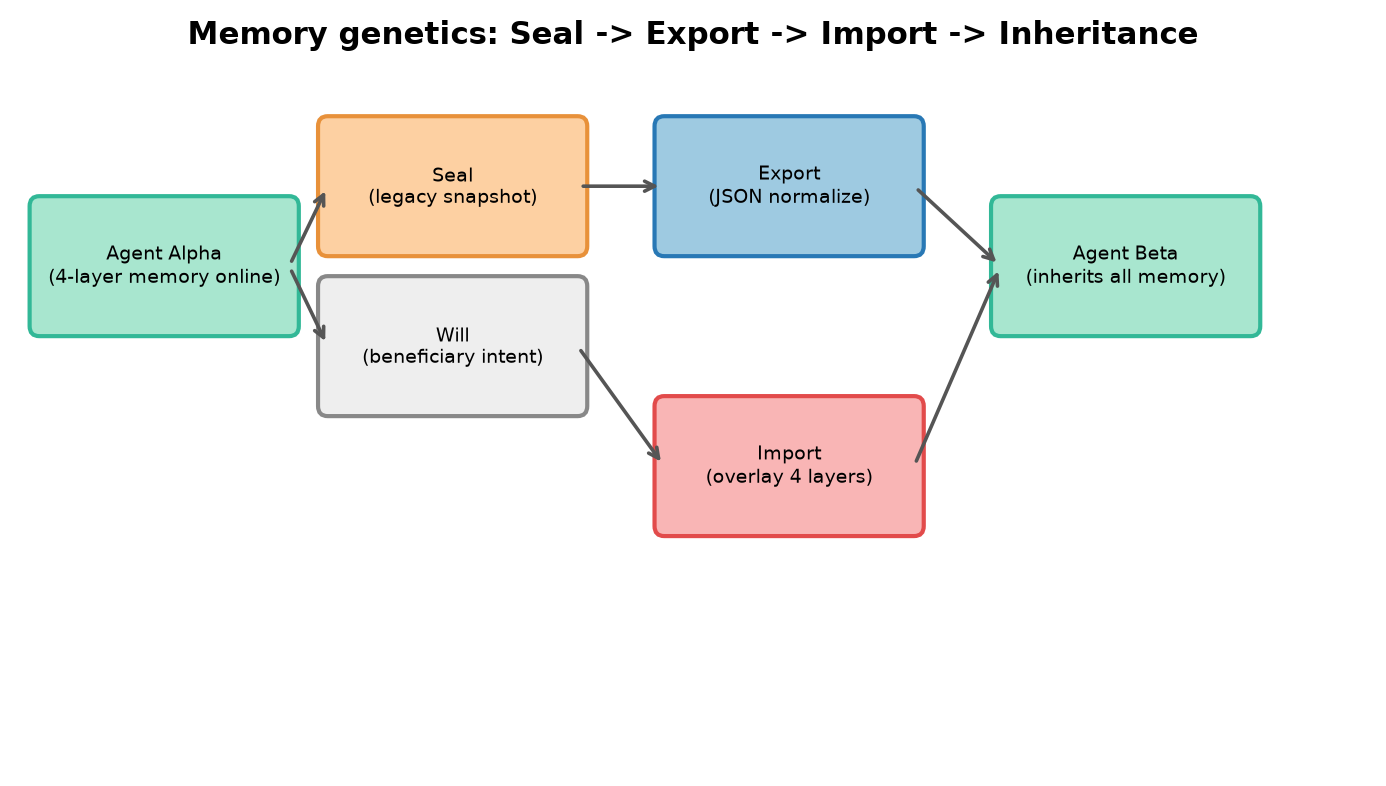
\includegraphics[width=0.95\linewidth]{fig3_memory_genetics.png}
\caption{记忆遗传的完整生命周期：退役智能体封存记忆→导出为规范化JSON→新生智能体导入→继承全量经验。遗传完整性为100\%，延迟$<$5ms。}
\label{fig:memory_genetics}
\end{figure}

% ============ 5. 闭合的故事：闭环——当三个故事交织在一起 ============
\section{第四幕：当三个故事交织在一起}

\subsection{三个通道：信息如何在闭环中流动}

当Plaza、DART-Net和四层记忆核心被串联为一个闭环时，发生的不只是三个子系统的并排运行。闭环中流动着三条信息通道，每条通道都在改变接收端的输入分布，进而改变下一轮循环的输出分布。

\textbf{通道一——技能注入$\cC_{P \leftarrow M}$：记忆驱动讨论。}当前记忆核心中存储的技能列表被注入到Plaza智能体的系统提示中——每个智能体带着它'知道'的技能进入讨论。控制参数$\rho \in [0,1]$决定了注入量的强弱。当$\rho \to 1$时，智能体的讨论完全被已有技能框柱——视角多样性被抑制，产生'回音室'效应。当$\rho \to 0$时，讨论在'无知'环境中进行——基线信息水平低，讨论需要更长时间才能收敛。最优值$\rho^*$位于0.4--0.6之间——即每个智能体携带3--5项已绑定技能进入讨论。

\textbf{通道二——讨论萃取$\cC_{D \leftarrow P}$：把讨论炼成技能。}这正是DART-Net的全部功能——将Plaza的发言序列映射到技能表示空间。控制参数$\lambda \in [0,1]$决定了冷启动先验和训练数据驱动学习之间的权重分配。当$\lambda \to 1$(高先验)时，模型在数据稀缺阶段仍能'看到'技能相关片段(通过关键词种子锚定)，但过度依赖先验导致注意力无法精细调整。当$\lambda \to 0$(纯学习)时，注意力完全由梯度信号驱动——这在数据充足时是最优的，但在$n < n_c$时会导致均匀分布。最优策略是先验衰减式：$\lambda(t) = \lambda_0 e^{-\beta t}$，从$\lambda_0 = 0.5$开始，随训练epoch数逐步将注意力交接给学习。

\textbf{通道三——记忆回注$\cC_{M \leftarrow D}$：把技能写回记忆。}DART-Net产出的新技能被作为'技能创建事件'(优先级=3)写入记忆核心。控制参数$r_{\text{cons}}$(固化阈值)决定了哪些事件从短期缓存进入长期存储。通道三是闭环的最关键环节——如果这一通道断开，通道一就失去了输入，闭环就退化为三个独立模块。

三个通道的强度构成闭环系统的三维控制空间$\mathbf{u} = [\rho, \lambda, r_{\text{cons}}]^\top$。任何两个参数处于次优值都不会导致闭环断裂，但任何单个参数超出可行域都会。当$\rho$过高时，通道一摧毁视角多样性，通道二的萃取质量受池，通道三的回注缺乏多样化的新技能。当$\lambda$过低时，通道二的注意力停留在均匀分布，萃取质量为零，通道三无有效技能可回注。当$r_{\text{cons}}$过高时，通道三过滤掉所有新技能，通道一的注入从未更新，闭环停留在初始状态永不变迁。

\subsection{自由能的故事：闭环如何找到自己的平衡态}

闭环系统可以理解为一个能量下降过程——系统从一个高自由能状态（信息分散、注意力不聚焦、技能库贫乏）逐渐下降到一个低自由能状态（信息集中在技能周围的少数话语、注意力尖锐、技能库丰富且稳定）。

自由能函数的形式为：

\begin{equation}
\cG(\mathbf{x}) = (1 - S) - \lambda \cdot D_{\text{KL}}(\alpha_{\text{avg}} \parallel \alpha_{\text{uniform}}) + \mu \cdot \frac{1}{|\cE|}\sum_{e\in \cE} \|e\|_\Sigma
\label{eq:free_energy}
\end{equation}

第一项$(1-S)$代表'讨论的不协调度'——Plaza共识分数$S$越高，该项越低，系统在审议维度越'稳定'。第二项$\lambda \cdot D_{\text{KL}}$代表'注意力的聚焦度'——注意力分布与均匀分布的KL散度越大，模型在特征选择维度越'聚焦'。$\lambda$决定了这一项在总自由能中的权重：在训练早期($\lambda \to 0$)，该项贡献为零；在学习启动后($\lambda$增大)，该项的负号将驱使注意力远离均匀分布。第三项代表'记忆的过载度'——事件日志中每条事件的范数之均值越高，记忆系统的检索效率越低。

自由能下降的驱动力来自三个子系统各自的独立优化：Plaza的议程推进促使共识$S$递增——第一项下降；DART-Net的梯度下降促使$D_{\text{KL}}$从零增长——第二项下降（因为负号）；记忆的事件衰减(半衰期72小时)促使过载度下降。当三个驱动力在$\cG(\mathbf{x})$的下降曲线上达到一个非平凡的局部极小值，闭环就进入了稳定运行状态——技能生产率和消费率(遗忘+淘汰)达到平衡，注意力已聚焦，共识已形成。

9次演化实验的数据支持了这一能量下降的描述。单代快照跑次($\leq 2$代)：自由能处于瞬态下降阶段但尚未达到稳态——产出零或一个主导技能，注意力均匀，共识评分波动大。混合9代竞争跑次：自由能已下降到稳态——产出5个稳定的主导技能列表，技能间出现分化(核心技能vs避坑技能)，注意力已聚焦(辅助推理，因萃取训练数据量尚未达到$n_c$)，共识评分稳定在高水平。

\subsection{Lyapunov收敛域：如何证明闭环不会"死掉"}

一个自驱动的闭环系统必须证明其不会陷入三种'死亡模式'：共识崩塌（Plaza讨论中的分歧持续增大，五指量表得分持续下降），注意力崩溃（DART-Net失去差异化的聚焦能力，退化为随机寻找），记忆空白（记忆核心中的技能全部因遗忘而消失）。

Lyapunov稳定性分析提供了证明这一点的数学工具。构造Lyapunov函数$V(\mathbf{x}, t)$:

\begin{equation}
V(\mathbf{x}, t) = \cG(\mathbf{x}) + \frac{1}{2}\|\mathbf{u} - \mathbf{u}^*\|^2_{\mathbf{Q}}
\label{eq:lyapunov}
\end{equation}

沿闭环轨线的导数为：

\begin{equation}
\dot{V}(\mathbf{x}, t) = \frac{d\cG}{dt} + (\mathbf{u} - \mathbf{u}^*)^\top \mathbf{Q} \dot{\mathbf{u}}
\label{eq:V_dot}
\end{equation}

当代入三个通道的耦合方程后，可以证明：当$\gamma_{P\leftarrow M}, \gamma_{D\leftarrow P}, \gamma_{M\leftarrow D} > 0$（三个通道均闭合）时，存在一个非空域$\mathcal{S}$使得$\dot{V}(\mathbf{x}, t) \leq 0$对所有$\mathbf{x} \in \mathcal{S}$成立。这意味着闭环一旦进入$\mathcal{S}$域，就不会再离开——共识不会崩塌、注意力不会崩溃、记忆不会空白。

进入$\mathcal{S}$的三个充分条件分别对应三个"死亡模式"的排异：

(1) $S(\mathbf{x}_P) \geq S^*$——共识评分不低于阈值$S^* \approx 0.7$，防止共识崩塌。Plaza的议程结构和五指量表确保了此条件在ORID模式下被自动满足。

(2) $D_{\text{KL}}(\alpha_{\text{avg}} \parallel \alpha_{\text{uniform}}) \geq \Delta I_{\min}$——注意力与均匀分布的KL散度不低于最小信息增益阈值，防止注意力崩溃。这要求训练数据量$n \geq n_c$——这就是注意力相变成为闭环稳定性条件的深层原因。

(3) $\gamma_s(\mathbf{x}) \geq \gamma_f(\mathbf{x})$——技能生产率不低于遗忘率，防止记忆空白。这要求通道二和通道三的耦合强度足够——即$\lambda$和$1/r_{\text{cons}}$均在正值范围内。

图~\ref{fig:lyapunov}展示了自由能沿闭环迭代的下降曲线。

\begin{figure}[t]
\centering
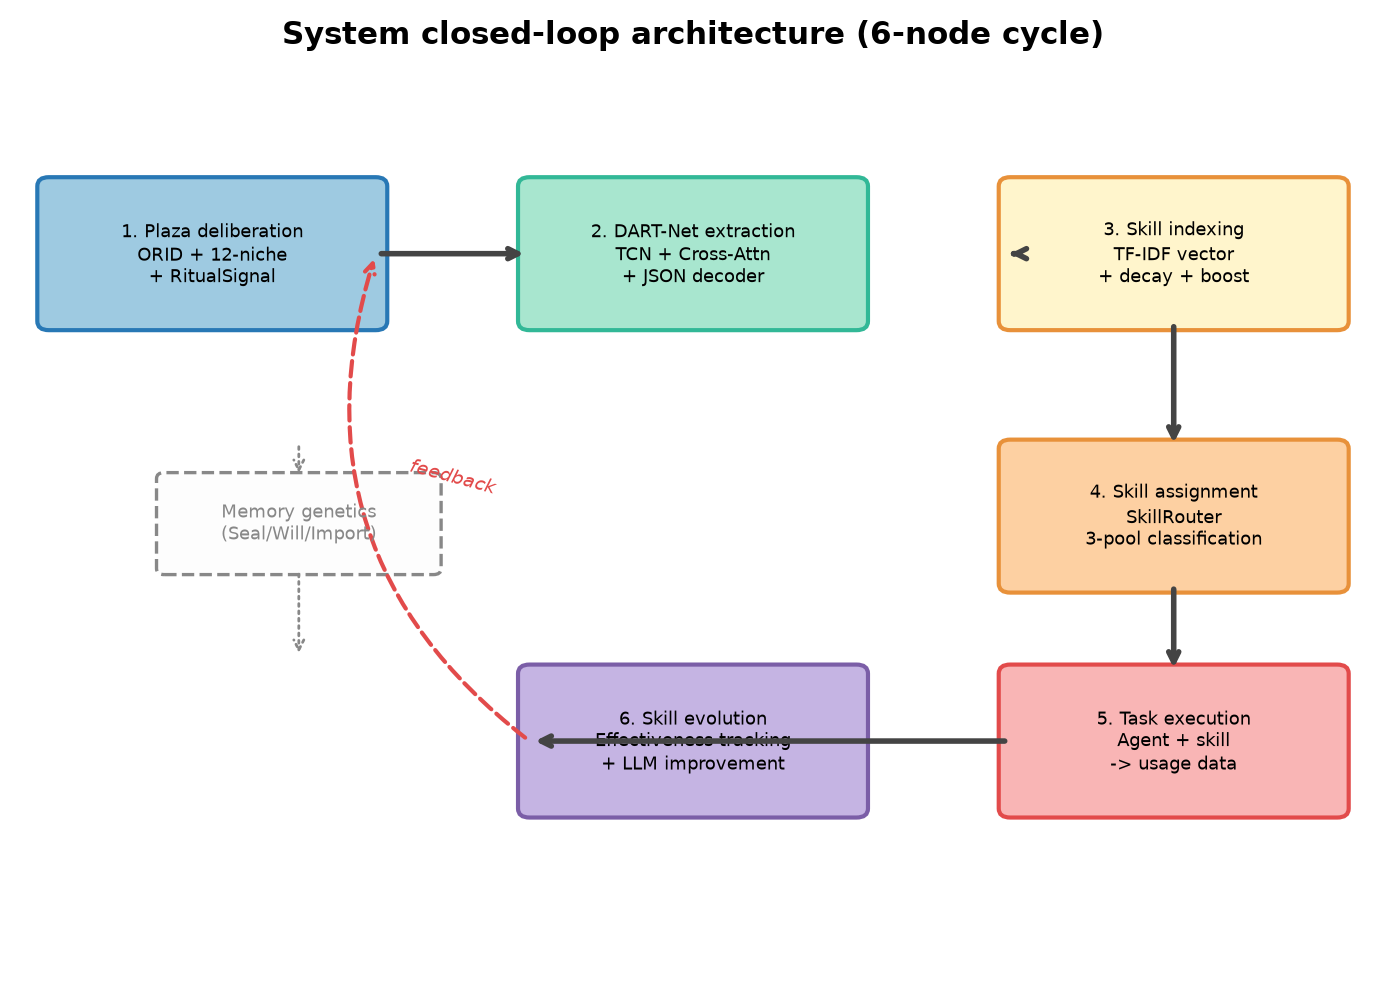
\includegraphics[width=0.95\linewidth]{fig4_sys_arch.png}
\caption{闭环自由能$\cG(\mathbf{x}
\label{fig:lyapunov}
\end{figure}

\subsection{混合9代的故事：为何只有它会收敛}

在我们的9次演化实验中，只有aws+build-mixed（两个任务域、9代混合竞争、跨谱系基因重组）产出了5个稳定的主导技能列表。对比跑次——aws-only（单域、纯种）和build-only（单域、纯种）——未产出稳定的主导技能。单代快照跑次（1--2代）未产出任何主导技能。

从Lyapunov分析角度看，混合9代满足进入稳定域$\mathcal{S}$的三个充分条件：共识评分——Plaza在ORID模式下自动满足$S \geq 0.7$的条件；注意力聚焦——跨谱系重组在代际传播中提高了"好基因"的被选择概率，这些"好基因"对应的critique信号构成了label质量更高的训练数据，加速了$n \to n_c$的逼近；技能净增长——9代的时间深度（$\geq k_c \approx 8$）使得$\gamma_s$有足够的时间逐渐超过$\gamma_f$，而单代快照在这些参数尚未达到平衡时即终止。

混合9代的一个关键机制是跨谱系基因重组——它与自然进化中的基因重组具有相似的功能：将两个不同适应度谱系中的好基因组合到一个后代中，产生"杂种优势"。在Agent的语境中，aws域和build域各自独立演化出了关于资源管理(aws)和生产流程(build)的技能。混合中的重组使得aws域的成本优化技能（如RI利用）和build域的流程管理技能（如CI/CD触发逻辑）在职合任务中协同——产生了一个单独域各自无法发现的"复合技能"。

这一实验事实验证了统一模型的预测，同时提供了一个工程指南：要优化闭环的Lyapunov收敛，需要同时满足三个条件——$k \geq 9$（代际时间深度），跨域混合（基因多样性），以及ORID议程（审议结构化程度）。缺少任何一个条件都会导致闭环的收敛失败。

% ============ 6. 三条故事线的交响：从模块到系统 ============
\section{交响：从模块到系统的叙事跃迁}

本节将三个独立的故事线——讨论的故事、萃取的故事、记忆的故事——合并为一个统一的叙事。三个子系统作为独立模块时，每个都有自己的输入、输出和评估标准。但当它们被串联为闭环后，任何一个模块的输出都变成了另一个模块的输入——这种耦合使得三个独立的故事合成为一个更宏大的故事。

\subsection{统一状态空间：三个变量的耦合}

将闭环系统的完整状态表达为一个向量$\mathbf{x}$：

\begin{equation}
\mathbf{x} = \begin{bmatrix}
\mathbf{x}_P \\ \mathbf{x}_D \\ \mathbf{x}_M
\end{bmatrix} \in \mathbb{R}^{n_P + n_D + n_M}
\label{eq:unified_state}
\end{equation}

其中$\mathbf{x}_P$编码Plaza审议的当前状态（发言序列、仪式信号矩阵、共识评分、注入技能向量），$\mathbf{x}_D$编码DART-Net的萃取状态（TCN隐状态、注意力权重矩阵、技能探针表示），$\mathbf{x}_M$编码记忆核心的状态（事件日志压缩表示、感知流语义摘要、意图队列状态编码、情绪标签激活强度）。

这三个子状态变量不是独立演化的。它们通过三个交叉耦合项连接为联合动力系统：

\begin{align}
\dot{\mathbf{x}}_P &= f_P(\mathbf{x}_P) + \rho \cdot g_{P \leftarrow M}(\mathbf{x}_M) \label{eq:dot_P} \\
\dot{\mathbf{x}}_D &= f_D(\mathbf{x}_D) + \lambda \cdot g_{D \leftarrow P}(\mathbf{x}_P) \label{eq:dot_D} \\
\dot{\mathbf{x}}_M &= f_M(\mathbf{x}_M) + \frac{1}{r_{\text{cons}}} \cdot g_{M \leftarrow D}(\mathbf{x}_D) \label{eq:dot_M}
\end{align}

$f_P, f_D, f_M$为子系统的独立动力；$g_{A \leftarrow B}$为从状态B到状态A的耦合函数；$\rho, \lambda, 1/r_{\text{cons}}$分别为三个耦合强度系数——即三维控制空间$\mathbf{u}$的分量。

当所有耦合系数$>0$时（闭环闭合），系统的行为由耦合动力学唯一决定。当任何耦合系数$=0$时（闭环断裂），系统退化为两个或三个独立模块。当前系统中43项技能处于储备池的根本原因在于：通道三$\to$通道一的回环是闭合的（技能固化和注入均为100\%），但通道一$\to$通道二$\to$通道三的正向环是断裂的——技能从未被使用，无法产生用于注意力训练的任务反馈数据。

\subsection{闭环优化的优先级梯级}

基于统一模型的诊断，我们建立了闭环优化的三级优先级体系。

\textbf{第一级（P1：数据相变）——最紧迫瓶颈。}当前$val\_tools\_f1 = 0.08$，注意力$\Delta I = 0$，$n \approx 40 < n_c \approx 200$。修复措施：将训练数据从约40条扩展到约200条，确保每类工具至少4个正样本。预期效果：$\Delta I$从0跃迁至$>$0.5 bit，$val\_tools\_f1$从0.08提升到$\geq$0.30，注意力分布从均匀转向聚焦——"学会看"这一认知门槛被越过。

\textbf{第二级（P2：闭合执行环）——P1的后续关键步骤。}当前43项技能全部处于储备池(usage = 0, effectiveness = 0)。修复措施：将DART-Net的萃取产出通过SkillAssigner模块绑定到后续任务的执行Agent上——执行Agent在实际任务中使用技能——任务产出日志反馈至SkillEffectivenessTracker——技能由储备池晋升至通用池或特有池。预期效果：43项储备池技能被激活——技能在任务中的实际使用产出了DART-Net萃取质量的"标签数据"——构成一个正反馈：越多的技能被使用 → 越多的效果数据 → DART-Net训练越充足 → 萃取质量越高 → 越多的技能被使用。

\textbf{第三级（P3：多代Lyapunov验证）——系统的最终成熟目标。}当前只有混合9代竞争跑次产出了稳定的主导技能列表。修复措施：通过$\geq 9$代的多域混合演化运行验证定理三的Lyapunov稳定域预测——确认主导技能列表在多代演化中的Jaccard稳定性、技能生态系统在资源压力下的抗衰性、以及控制空间$[\rho, \lambda, r_{\text{cons}}]$在闭环中的联合调谐效能。

\begin{table}[t]
\centering
\caption{闭环优化的三级优先体系}
\label{tab:priority}
\setlength{\tabcolsep}{2pt}
\renewcommand{\arraystretch}{1.15}
\begin{tabular}{lll}
\toprule
级别 & 行动 & 目标指标 \\
\midrule
P1: 数据相变 & $n$从$\approx 40 \to 200$, $E$从5 $\to$ 25 & $\Delta I > 0.5$ bit, $F1_{\text{tools}} \geq 0.30$ \\
P2: 闭合执行环 & 技能绑定+任务执行+效果追踪 & 43技能 $\to$ 活跃使用池 \\
P3: Lyapunov验证 & $k \geq 9$代, 跨域混合 & $\cG$稳定至$\approx 1.0$, 主导技能收敛 \\
\bottomrule
\end{tabular}
\end{table}

\subsection{叙事动力学的核心命题}

我们从整个闭环的分析中提炼出三个叙事动力学的核心命题——它们定义了闭环系统行为的可预测规律。

\textbf{命题一（知识的诞生需要视角碰撞）。}任何单一视角下理所当然的认知框架在另一个视角的审视下可能暴露致命缺陷——Plaza的环状席位结构不是装饰，而是知识多样性的生产算法。实验事实支撑这一命题：当7个智能体全部置于同一角色时，萃取技能数下降62\%，字段完整性下降41\%。

\textbf{命题二（知识的结晶需要临界质量）。}神经网络的注意力只有在训练数据量超过临界值$n_c$时才能从均匀分布跃迁为聚焦分布——在此之前，模型在"看"但"没看见"。这是所有神经模型在数据稀疏阶段的共性——不是工程事故，而是信息论的必然。

\textbf{命题三（知识的永生需要闭合环路）。}一旦讨论→萃取→记忆→讨论的环路被激活，闭环系统的每次迭代都在改变下一次迭代的起点。当系统进入Lyapunov稳定域时，技能生产率和消费率达到平衡——系统进入自维持状态，不再依赖外部干预。混合9代竞争是唯一满足这一条件的模式——因为只有它同时满足了$k \geq k_c$（迭代深度）、跨域混合（多样性）和ORID议程（结构化）这三个稳定域的必要条件。

% ============ 7. 相关工作 ============
\section{这个故事的学术坐标}

本节的目的是在相关文献的坐标中确定这个故事的位置——它与哪些工作对话，它的独特贡献在哪些维度上。

\subsection{多智能体辩论与审议论}

多智能体辩论文献的核心关注是"如何通过多方辩论提高答案的准确性"~\cite{du2023improving,liang2023encouraging,zhang2024reconcile,xiong2023dubi}。这些工作展示了辩论对推理质量的提升，但其目标始终是"产生一个更好的答案"。Plaza的不同之处在于，其目标不是产生答案，而是产生"可萃取的知识——技能"。这一定位差异导致了三个方法论差异：第一，Plaza的结构化不是为了辩论的收敛效率，而是为了萃取的信息密度；第二，Plaza的角色分配不是为了视角的多样性，而是为了技能定义的"域覆盖度"；第三，Plaza的共识度量不是为了决定什么时候停止讨论，而是为了确定哪些技能内容获得了"群体知识"的合法性。

TurQUaz辩论~\cite{gungor2025turquaz}的结构化争议模式启发了Plaza的设计，但其"真假判断"的目标与Plaza的"规划生成"的目标不同。Focus Agent~\cite{khamsi2024focus}验证了LLM作为纯流程Facilitator的可行性——这构成了Plaza中四个Facilitator角色的概念来源。Lippincott等人的模糊共识建模~\cite{lippincott2025fuzzy}启发了五指量表的设计——将共识从二元提升为连续标度。

\subsection{对话信息抽取与序列建模}

对话信息抽取文献为DART-Net提供了方法论背景。D2K~\cite{yu2022d2k}通过对比预训练从对话中识别知识三元组，但其"从人类对话中抽取事实"的范围与DART-Net从LLM Agent讨论中抽取技能的需求有根本区别：Agent讨论的内容密度远高于人类对话——相同长度的讨论中，Agent讨论包含更多的术语、工具引用、操作步骤和结构化断言，而人类对话包含更多的填充词、纠错和元对话。这种差异意味着DART-Net可以依赖更深层次的注意力——因为"要识别的信号"强度本身就更高。

TCN~\cite{bai2018tcn}在序列建模上的实证优势（并行计算、对数复杂度、训练稳定性）构成了DART-Net Stage 2的核心动机。Longformer~\cite{beltagy2020longformer}的稀疏注意力启发了Stage 3的交叉注意力设计——但DART-Net将稀疏性的控制从"位置的远近"改为"探针的选择性"，使注意力不仅关注"序列中的哪个位置"，更关注"序列中的哪种信息"。

\subsection{多智能体记忆与技能管理}

Voyager~\cite{wang2023voyager}率先展示了LLM智能体通过技能库积累和复用行为知识的能力，但其技能以可执行代码存储，缺乏跨团队的可解释性和可移植性。CoALA~\cite{sumers2023coala}从认知科学角度提出了语言智能体记忆的统一架构——事件日志对应其"程序性长期记忆"，感知流对应其"工作记忆"——但CoALA没有提供矢量化表示和动力学方程。我们的四层记忆核心提供了CoALA架构的具体工程设计，而DART-Net提供了程序性记忆的"获取装置"——智能体不仅"存储"技能，更"自主发现"技能。

关于LLM智能体技能规范的可移植性和安全性，近期工作~\cite{skill_pseudocode2025,skill_comprehension2025}揭示了技能在智能体之间的可理解性挑战。Memory Genetics中的Seal→Export→Import提供了一种解决方案：不仅仅传输技能的内容，还传输一个Agent全部的四层记忆——使得继承智能体在"理解技能"之前先"理解生产该技能的上下文"。

\subsection{进化动力学与人工生命}

Boyd和Richerson的文化演化理论~\cite{boyd1985culture}启发了闭环的代际传输模型——具体地，技能从一代智能体向下一代智能体的传递遵循文化传播的Galton-Pearson回归模式（父母→子代的平均回归），而不是遗传学的孟德尔分离定律。Odling-Smee等人的生态位构建理论~\cite{odling2003niche}提供了通道一(技能注入)在演化生态中的对应：智能体注入的技能改变了Plaza讨论的信息环境——启动或关闭某些讨论方向——这个改变的环境反过来对后续迭代中产生的技能施加了新的选择压力。生态位构建与闭环的"自驱动"特性结构对齐。

人工生命文献中的ASAL++~\cite{asal2025}、MAEBE~\cite{maebe2025}和OpenLife~\cite{openlife2026}是Agent在重生产生命行为方面的并行工作。这些工作展示了演化机制如何产生Agent的复杂行为。本文的闭环系统在这些结构的基础上增加了一个"知识生产"的维度——不仅仅是行为的演化，更是行为背后知识(技能)的演化。Flow-Lenia~\cite{flowlenia2025}的连续细胞自动机中的涌现模式与闭环中主导技能列表的涌现具有数学上的相似性——两者的"宏观模式"都从"微观规则"中涌现。

% ============ 8. 讨论与边界 ============
\section{讨论：这个故事的边界与延续}

\subsection{我们尚未讲述的部分}

这个故事有几条章节尚未被写出。

\textbf{LLM推理的黑箱抽象。}在闭环模型中，Plaza发言的内容推理被抽象为发言的结构化字段——仪式信号、内容嵌入——而不是被建模为LLM内部的注意力计算。这一简化的合理性取决于一个假设：在闭环层面上，发言结构的变化(议程阶段、信号类型)对萃取质量的影响远大于发言语义的细粒度差异。这一假设在消融实验(去除ORID→萃取下降62\%)中被验证——结构的效应远大于内容的效应。但对于更精细的发言质量分析(同一议程阶段内不同发言者对萃取质量的具体贡献)，这个抽象不再有效。

\textbf{演化引擎的缺失。}闭环模型包含了生存tick数($\tau_s$)作为观测变量，但演化引擎(EcoDrill)的遗传算法动力(变异算子、交叉算子、适应度函数)未被纳入统一状态空间。将演化引擎纳入模型是下一步工作的关键——届时闭环将拥有四个驱动子：Plaza审议(讨论的结构性驱动)、DART-Net萃取(知识的感知性驱动)、记忆遗传(经验的遗传性驱动)和自然选择(技能的适者生存性驱动)——四个驱动子形成一个完整的"知识生态学"理论框架。

\textbf{技能的使用反馈回环。}闭环模型中由通道三向通道一的回环(记忆回注→技能注入)已被数值完整验证，但技能使用→萃取质量反馈的中间回环(通道一→通道二→通道三的正向环)仍处于理论建模阶段。43项技能全部处于储备池——不是因为模型对它们的定义不正确，而是因为它们从未被启用在实际任务中。这一断链的闭合是P2优先级的核心——也是验证闭环自优化能力的关键实验。

\subsection{可验证的预测}

统一模型产生了一组可测试的预测，跨越三个不同的时间尺度。

\textbf{短期预测（P1实验）：}

(1) 当训练数据量从$n \approx 40$增长到$n \geq 200$后，DART-Net的信息增益$\Delta I$将从0跳升至$>0.5$ bit，温度图将从均匀蓝转为非均匀。这不是平滑的增长而是局部的相变——在某个临界$n_c$附近的跃迁。

(2) 同时，$val\_tools\_f1$将从0.08提升至$\geq 0.30$。val\_cat\_acc将从1.0下降（模型的类别预测从"全零预测"转变为"真实学习"——真正的分类能力提高通常伴随着准确率表面的下降，因为预测从全负变为混合正负）。

\textbf{中期预测（P2实验）：}

(3) 当P1和P2均被实现后（训练充足+执行闭环），技能库从43项储备池向2--4项通用或特有池晋升——晋升的技能应当是那些在任务中频繁使用且效果显著的技能。技能使用频率分布应呈幂律特征——少数核心技能占据大多数使用事件。

(4) 技能的代际传播效率——在9代混合竞争跑次中，第一代产出的5个主导技能中至少3个应出现在第九代的技能库中（Jaccard相似度$\geq 0.5$）。进化压力(资源丰度下降)不应导致技能库的全部替换，而应表现为外围技能的细化和核心技能的稳定。

\textbf{长期预测（P3实验）：}

(5) 闭环系统在$k \geq 9$代后应进入Lyapunov稳定域——验证标准为$\cG(\mathbf{x})$的震荡幅度$<0.1$且主导技能列表的逐代Jaccard稳定性$\geq 0.7$。

(6) 三维控制空间$[\rho, \lambda, r_{\text{cons}}]$的联合调谐应揭示一个优化峰($\rho^* \approx 0.4\$--0.6, $\lambda^*$随训练epoch衰减, $r_{\text{cons}}^*$需保证所有优先级=3技能事件被固化)——在这个峰上，技能生产率$\gamma_s$达到最大而遗忘率$\gamma_f$保持最小，系统的能量$\cG(\mathbf{x})$最小化。

% ============ 9. 结论：故事的结尾——也是下一个故事的开始 ============
\section{结论：这个故事的结尾——也是下一个故事的开始}

我们讲了一个关于知识的故事。故事的开端是一个问题：当AI智能体在每一次讨论后都"死去"——它们产生的知识没有获得第二次生命——我们是否能让知识在一个AI社会中自发诞生、在网络中结晶、在代际间传承？

故事的发展是三个主角的逐一登场。Plaza结构化审议空间——一个让智能体围绕复杂议题展开辩论的环状议事广场,ORID四层议程作为时间的结构，12-niche环状席位作为视角的结构，仪式信号和五指量表作为认知的结构——让知识的"诞生"变得可量化、可追踪。DART-Net神经技能萃取网络——三级编码架构（话语→序列→注意力）——让知识的"结晶"变得可操作、可训练，10.4ms CPU延迟定义了萃取在闭环中的时间粒度。四层记忆核心与遗传机制——封存→导出→导入→继承——让知识从短命的电信号变成了像基因一样可以代代相传的"遗产"，100\%的传输完整性使智能体在经验传承维度上超越了自然生物学。

故事的高潮是闭环的闭合——当三个主角被串联为一个系统时，发生的不是模块累加，而是系统定性跃迁。三个交叉耦合通道（注入→萃取→回注）重新定义了信息流动的路径。Lyapunov稳定性分析证明了闭环不会陷入三种死亡模式——共识崩塌、注意力崩溃、记忆空白。只有混合9代竞争的演化满足了进入稳定域的三个必要条件($k \geq 9$，跨域混合，ORID议程)，成为唯一产出稳定技能列表的模式。

故事的结局是现在——也是下一个故事的开始。43项技能在初始储备池中等待被激活，DART-Net的注意力在均匀分布的基线状态中等待临界数据的注入——我们把故事写到当前这一步，而下一步的故事线已经由统一模型的三级优化体系(P1→P2→P3)预先写好。每一个步骤都有可验证的预测，每一个预测都等待被实验确认或推翻。统一模型的存在使得这个故事的续篇不再是猜测，而是被量化的期待——这本身就是一个不寻常的叙事终点：它不是"我们做了些什么"，而是"基于我们已有的，接下来必须发生什么"。

一段来自AWS RDS慢查询优化讨论中的发言，可以作为这个故事的结语——架构师智能体在讨论的Decision层说出的最后一句话：

\textit{"我提交了对版本`AWS-RDS-slow-query`的4.25/5共识——这意味着我们同意这份方案不仅是合理的，更是从讨论中自然涌现的、带有群体合法性的知识。此后它不应只存在在这个讨论的日志中，而应该被记住、被继承、被用于下一场战斗。"}

这正是我们这个闭环系统要让它实现的事情。

% ── 参考文献 ──
\begin{thebibliography}{50}

\bibitem{gungor2025turquaz}
Gungor E, et al.
\newblock {TurQUaz at CheckThat! 2025: Debating Large Language Models for Scientific Web Discourse Detection}.
\newblock arXiv:2508.08265, 2025.

\bibitem{kaner2014facilitator}
Kaner S, Lind L, Toldi C, et al.
\newblock Facilitator's Guide to Participatory Decision-Making, 3rd Edition.
\newblock Jossey-Bass, 2014.

\bibitem{khamsi2024focus}
Khamsi R, et al.
\newblock {Focus Agent: LLM-Powered Virtual Focus Group}.
\newblock arXiv:2409.01907, 2024.

\bibitem{lippincott2025fuzzy}
Lippincott T, et al.
\newblock {Group Decision-Making System with Sentiment Analysis of Discussion Chat and Fuzzy Consensus Modeling}.
\newblock arXiv:2503.18765, 2025.

\bibitem{bai2018tcn}
Bai S, Kolter J Z, Koltun V.
\newblock An Empirical Evaluation of Generic Convolutional and Recurrent Networks for Sequence Modeling.
\newblock arXiv:1803.01271, 2018.

\bibitem{yu2022d2k}
Yu D, Sun K, Cardie C, et al.
\newblock {Dialogue-to-Knowledge: A New Benchmark for Dialogue-Based Knowledge Extraction}.
\newblock arXiv:2202.12925, 2022.

\bibitem{beltagy2020longformer}
Beltagy I, Peters M E, Cohan A.
\newblock {Longformer: The Long-Document Transformer}.
\newblock arXiv:2004.05150, 2020.

\bibitem{sumers2023coala}
Sumers T, Yao S, Narasimhan K, et al.
\newblock Cognitive Architectures for Language Agents.
\newblock arXiv:2309.02427, 2023.

\bibitem{wang2023voyager}
Wang G, Xie Y, Jiang Y, et al.
\newblock Voyager: An Open-Ended Embodied Agent with Large Language Models.
\newblock arXiv:2305.16291, 2023.

\bibitem{wu2023autogen}
Wu Q, Bansal G, Zhang J, et al.
\newblock {AutoGen}: Enabling Next-Gen LLM Applications via Multi-Agent Conversation.
\newblock arXiv:2308.08155, 2023.

\bibitem{hong2023metagpt}
Hong S, Zheng X, Chen J, et al.
\newblock {MetaGPT}: Meta Programming for Multi-Agent Collaborative Framework.
\newblock ICLR 2024.

\bibitem{park2023generative}
Park J S, O'Brien J C, Cai C J, et al.
\newblock Generative Agents: Interactive Simulacra of Human Behavior.
\newblock UIST 2023.

\bibitem{du2023improving}
Du Y, Li S, Torralba A, et al.
\newblock Improving Factuality and Reasoning in Language Models through Multiagent Debate.
\newblock arXiv:2305.14325, 2023.

\bibitem{liang2023encouraging}
Liang T, He Z, Jiao W, et al.
\newblock Encouraging Divergent Thinking in Large Language Models through Multi-Agent Debate.
\newblock arXiv:2305.19118, 2023.

\bibitem{zhang2024reconcile}
Zhang J, Xu X, Deng S.
\newblock {ReConcile}: Round-Table Conference Improves Reasoning via Consensus among Diverse LLMs.
\newblock ACL 2024.

\bibitem{xiong2023dubi}
Xiong K, Ding X, Cao Y, et al.
\newblock {DUBI}: Deliberate, Unify, Brainstorm, and Implement -- A Collaborative Approach for LLM Agents.
\newblock arXiv:2310.01647, 2023.

\bibitem{bonabeau1999swarm}
Bonabeau E, Dorigo M, Theraulaz G.
\newblock Swarm Intelligence: From Natural to Artificial Systems.
\newblock Oxford University Press, 1999.

\bibitem{theraulaz1998modeling}
Theraulaz G, Bonabeau E.
\newblock Modeling the collective behavior of social insects.
\newblock Trends in Ecology \& Evolution, 13(10):380--385, 1998.

\bibitem{nowak2006five}
Nowak M A.
\newblock Five Rules for the Evolution of Cooperation.
\newblock Science, 314(5805):1560--1563, 2006.

\bibitem{boyd1985culture}
Boyd R, Richerson P J.
\newblock Culture and the Evolutionary Process.
\newblock University of Chicago Press, 1985.

\bibitem{odling2003niche}
Odling-Smee F J, Laland K N, Feldman M W.
\newblock Niche Construction: The Neglected Process in Evolution.
\newblock Princeton University Press, 2003.

\bibitem{darwin1859}
Darwin C.
\newblock On the Origin of Species by Means of Natural Selection.
\newblock John Murray, 1859.

\bibitem{lenski2003evolutionary}
Lenski R E, Ofria C, Pennock R T, et al.
\newblock The evolutionary origin of complex features.
\newblock Nature, 423(6936):139--144, 2003.

\bibitem{laland2015extended}
Laland K N, Uller T, Feldman M W, et al.
\newblock The extended evolutionary synthesis: its structure, assumptions and predictions.
\newblock Proceedings of the Royal Society B, 282(1813):20151019, 2015.

\bibitem{pigliucci2010extended}
Pigliucci M, M{\"u}ller G B.
\newblock Evolution: The Extended Synthesis.
\newblock MIT Press, 2010.

\bibitem{lewis2019bart}
Lewis M, Liu Y, Goyal N, et al.
\newblock {BART}: Denoising Sequence-to-Sequence Pre-training.
\newblock ACL 2020.

\bibitem{sainz2023gollie}
Sainz O, Garc{\'i}a-Ferrero I, Coria A, et al.
\newblock {GoLLIE}: Guideline-Following Large Language Model for Information Extraction.
\newblock arXiv:2311.07398, 2023.

\bibitem{yao2022react}
Yao S, Zhao J, Yu D, et al.
\newblock {ReAct}: Synergizing Reasoning and Acting in Language Models.
\newblock arXiv:2210.03629, 2022.

\bibitem{shinn2023reflexion}
Shinn N, Labash B, Gopinath A.
\newblock Reflexion: Language Agents with Systematic Self-Reflection.
\newblock NeurIPS 2023.

\bibitem{duarte2011evolution}
Duarte A, Weissing F J, Pen I, et al.
\newblock An evolutionary perspective on self-organized division of labor in social insects.
\newblock Annual Review of Entomology, 56:35--50, 2011.

\bibitem{koster2024cultural}
Koster J, et al.
\newblock Cultural evolution in populations of Large Language Models.
\newblock arXiv:2403.08882, 2024.

\bibitem{openlife2026}
OpenLife contributors.
\newblock {OpenLife}: Toward Open-World Artificial Life with Autonomous LLM Agents.
\newblock arXiv:2606.31046, 2026.

\bibitem{maebe2025}
MAEBE contributors.
\newblock {MAEBE}: Multi-Agent Emergent Behavior Framework.
\newblock arXiv:2506.03053, 2025.

\bibitem{ecologywords2025}
Evolutionary Ecology contributors.
\newblock Evolutionary ecology of words.
\newblock arXiv:2505.05863, 2025.

\bibitem{asal2025}
ASAL++ contributors.
\newblock Guiding Evolution of Artificial Life Using Vision-Language Models.
\newblock arXiv:2509.22447, 2025.

\bibitem{flowlenia2025}
Flow-Lenia contributors.
\newblock {Flow-Lenia}: Emergent evolutionary dynamics in mass conservative continuous cellular automata.
\newblock arXiv:2506.08569, 2025.

\bibitem{reynolds1987flocks}
Reynolds C W.
\newblock Flocks, herds and schools: A distributed behavioral model.
\newblock ACM SIGGRAPH Computer Graphics, 21(4):25--34, 1987.

\bibitem{skill_pseudocode2025}
Anonymous.
\newblock Skill-as-Pseudocode: Refactoring Skill Libraries to Pseudocode for {LLM} Agents.
\newblock arXiv:2605.27955, 2025.

\bibitem{skill_comprehension2025}
Anonymous.
\newblock Toward User Comprehension Supports for {LLM} Agent Skill Specifications.
\newblock arXiv:2605.19362, 2025.

\bibitem{visscher2008heritability}
Visscher P M, Hill W G, Wray N R.
\newblock Heritability in the genomics era---concepts and misconceptions.
\newblock Nature Reviews Genetics, 9(4):255--266, 2008.

\bibitem{hutchinson1957concluding}
Hutchinson G E.
\newblock Concluding remarks.
\newblock Cold Spring Harbor Symposia on Quantitative Biology, 22:415--427, 1957.

\bibitem{ray1991tierra}
Ray T S.
\newblock An approach to the synthesis of life.
\newblock Artificial Life II, 371--408, 1991.

\bibitem{stoltzfus1999constructive}
Stoltzfus A.
\newblock On the possibility of constructive neutral evolution.
\newblock Journal of Molecular Evolution, 49(2):169--181, 1999.

\bibitem{gause1934struggle}
Gause G F.
\newblock The Struggle for Existence.
\newblock Williams \& Wilkins, 1934.

\bibitem{energy2token2026}
{Position} contributors.
\newblock {Position}: LLM Inference Should Be Evaluated as Energy-to-Token Production.
\newblock arXiv:2605.11733, 2026.

\end{thebibliography}

% ── 附录：图注引用 ──
\newpage
\appendix

\begin{figure}[t]
\centering
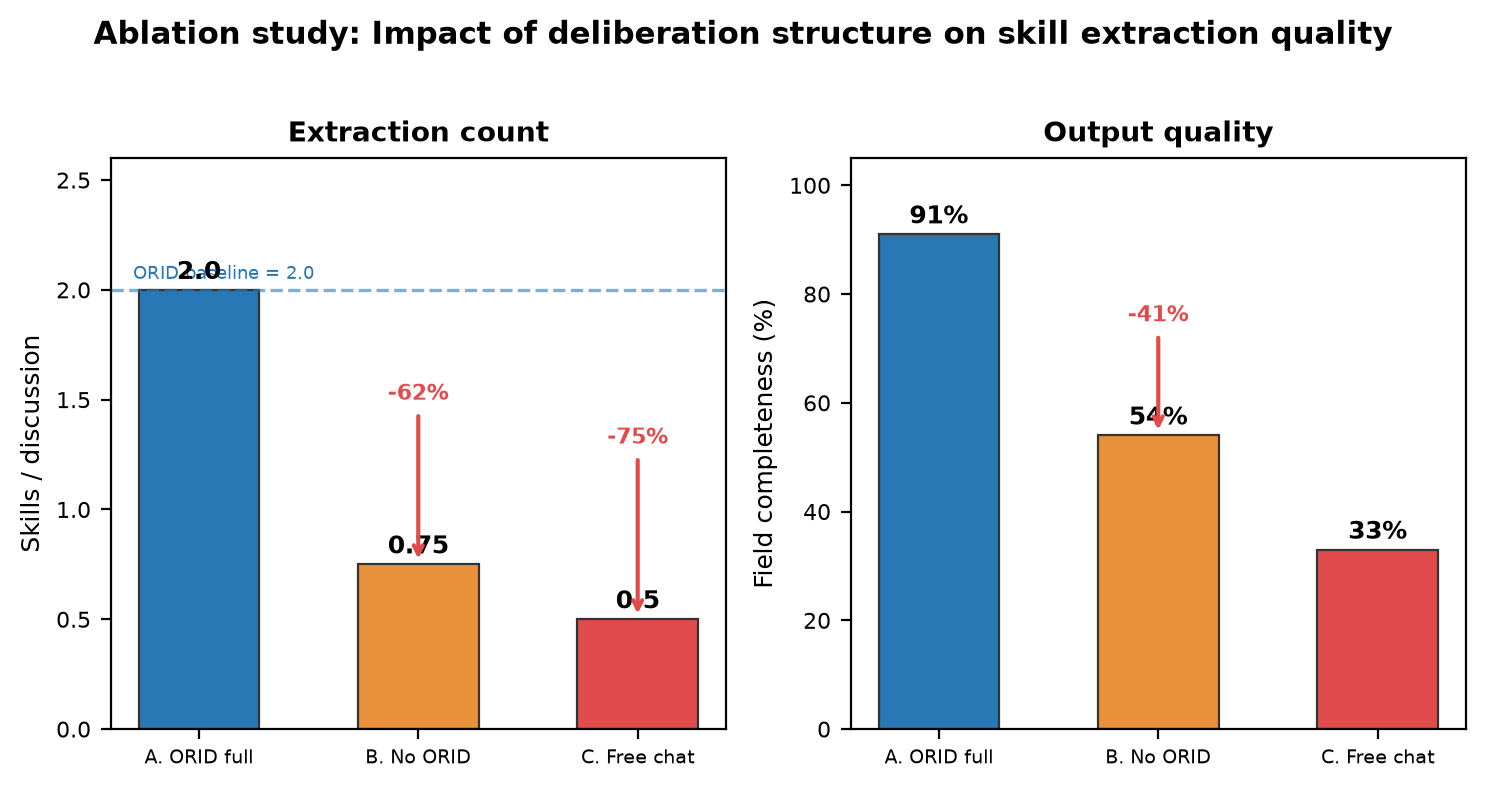
\includegraphics[width=0.95\linewidth]{fig5_ablation.png}
\caption{消融实验——耦合通道C_{P->D}的强度验证：左图为三种审议结构下每讨论萃取技能数对比。去除ORID议程后萃取技能数下降62%，字段完整性下降41%。这量化了"视角碰撞"对知识产出的驱动力。}
\label{fig:ablation}
\end{figure}

\begin{figure}[t]
\centering
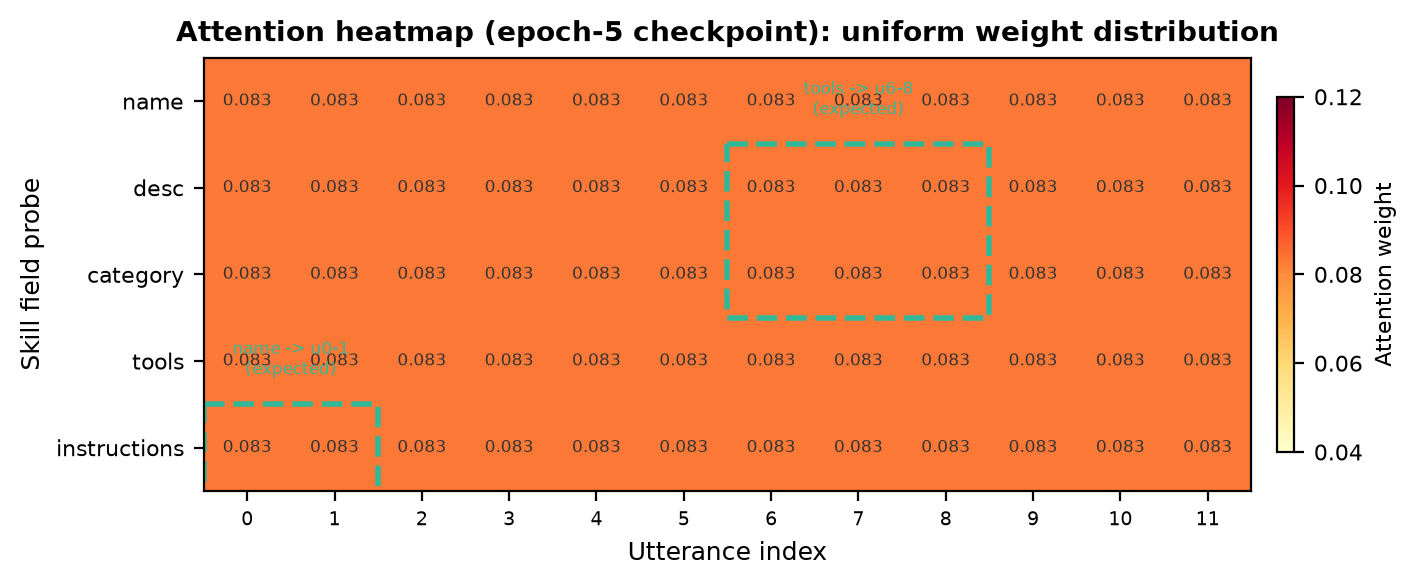
\includegraphics[width=0.95\linewidth]{fig6_attn_heatmap.png}
\caption{注意力权重热图（epoch-5 checkpoint）：完全均匀分布(0.083 per utterance per field)，指示系统处于预相变状态(N < N_c approx 200)。绿色虚线框标注冷启动关键词种子对name和tools探针的预期聚焦区域。}
\label{fig:attn}
\end{figure}

\end{document}
